%%%%%%%%%%%%%%%%%%%%%%%%%%%%%%%%%%%%%%%%%%%%%%%%%%%%%%%%%%%%%%%%%%
%%         mmm  mmmmmm mm   m        m    m mmmmmm  mmmm        %% 
%%       m"   " #      #"m  #        #    # #      "   "#       %%
%%       #   mm #mmmmm # #m #        #    # #mmmmm     m"       %%
%%       #    # #      #  # #  """   #    # #        m"         %%
%%        "mmm" #mmmmm #   ##        "mmmm" #mmmmm m#mmmm       %%
%%                                                              %%
%%                                                              %%
%%      Grundlagen der Elektrischen Netzwerke, UE               %%
%%      Gruppe 5, Team F                                        %%
%%      Authors: Severin Wolf, Maximilian Seidler.              %%
%%%%%%%%%%%%%%%%%%%%%%%%%%%%%%%%%%%%%%%%%%%%%%%%%%%%%%%%%%%%%%%%%%
\documentclass[a4paper]{article}
\usepackage{amsmath}
\usepackage[utf8]{inputenc}
\usepackage[T1]{fontenc}
\usepackage[english]{babel}
\usepackage{geometry}
\usepackage{graphicx}
\usepackage{tikz}
\usepackage{listings}
\geometry{a4paper,left=3cm,right=2cm, top=2cm, bottom=2cm} 
\usepackage[EFvoltages, european, straightvoltages]{circuitikz}

%tikz
\ctikzset{resistor = european}
\usetikzlibrary{decorations.pathreplacing}

%no paragraph indent
\setlength{\parindent}{0pt}

%for math, that does not fit
\renewcommand*{\arraystretch}{1.3}
\newcommand\scalemath[2]{\scalebox{#1}{\mbox{\ensuremath{\displaystyle #2}}}}

\newcommand\blfootnote[1]{%
	\begingroup
	\renewcommand\thefootnote{}\footnote{#1}%
	\addtocounter{footnote}{-1}%
	\endgroup
}

\begin{document}
\pagestyle{empty} \enlargethispage*{25cm}\samepage{
\vspace*{-3cm}
\begin{center}
\begin{minipage}[!h]{16cm}
\hspace*{0.2cm}

\includegraphics[width=3.3cm]{./Figures/igte_logo}
\begin{tabular}{p{8cm}}
\vspace{0.2cm}
\centering{
\Large Institute of Fundamentals and Theory in
 Electrical Engineering\\
Graz University of Technology\\
~\\}
\end{tabular}

\includegraphics[width=3.3cm]{./Figures/TUG_logo}
\end{minipage}
		\Large
		\textbf{Fundamentals of electrical circuits} \vspace*{0.5cm}\\
		\textbf{2. Homework}\\Th$\acute{\text{e}}$venin Equivalent Circuit and Linearity
		\vspace*{0.5cm}
		
		\large
		18 March 2021
	\end{center}}
	
	\vspace*{1cm}
	
	%%%%%%%%%%%%%%%%%%%%%%%%%%%%%%%%%%%%%%%%%%%%%%%%%%%%%%%%%%%%%%%%%%%%
	%%%%%%%%%%%%%%%%%%%%%%%%%%%%%%%%%%%%%%%%%%%%%%%%%%%%%%%%%%%%%%%%%%%%
	\section{Assignment 1}
	Consider the following circuit. The voltage source $U_{S1}$ is a \textbf{current-controlled voltage source}.\\
	The Th$\acute{\text{e}}$venin equivalent should be determined for the circuit on the left hand side with respect to the terminals \textbf{(a,b)} by using the \textbf{\textcolor[rgb]{1,0,0}{modified} node voltage method}.
	\begin{enumerate}
		\item  Mark the currents and voltages across every element, the missing nodes and all node-voltages in the part of the circuit to be replaced. (0.5P)
		\item Find the Th$\acute{\text{e}}$venin equivalent circuit with respect to the terminals $\mathbf{a}$ and $\mathbf{b}$ representing the left hand side of the circuit ($U_{Th}$,$R_{Th}$). (3P)
		\begin{itemize} 
			\item Therefor apply the modified node voltage method to the part of the circuit to be replaced. The matrix should be determined by inspection. Explain your thoughts briefly in the protocol (equations are not necessary). Write down the additional conditions needed to solve the system of equations. Solve the system of equations in matrix form $\mathbf{A}\cdot \mathbf{x} = \mathbf{b}$ (include the results!) in Matlab and determine the open-circuit voltage $U_{\text{oc}}$ at the terminals $\mathbf{a}$ and $\mathbf{b}$.
			\item Apply a test voltage $U_T$ in order to calculate the Th$\acute{\text{e}}$venin resistance $R_{Th}$. \\
			\textbf{Hint1:} Each independent source can be deactivated in LTspice by simply setting its value to 0. No additional changes to the circuit are needed.
		\end{itemize}
		\item Confirm the calculated results for $U_{Th}$ and $R_{Th}$ in LTspice. Simulate both circuits. In order to confirm that the the Th$\acute{\text{e}}$venin equivalent circuit and the original circuit are equivalent to each other, make a simulation of the original circuit and the one with the calculated Th$\acute{\text{e}}$venin equivalent. Compare the results. Overall four simulations are needed. (1.5P)		
	\end{enumerate} 
			\textbf{2P Bonus:}
			\begin{itemize} 
				\item Draw the given circuit with the previously calculated Th$\acute{\text{e}}$venin equivalent circuit on the left hand side.
				\item Adjust the value of the current source $I_{S3,\text{new}}$ so that the voltage across the resistor $R_6$ equals $U_{R_6,\text{new}}=20V$ and confirm your result in LTspice.
			\end{itemize}
\vspace*{3.5cm}
	\subsection*{Values:}
	$R_1 = 10\Omega$ \qquad $R_2 = 5\Omega$ \qquad $R_3 = 8\Omega$ \qquad $R_4 = 12\Omega$ \qquad $R_5 = 6\Omega$ \qquad $R_6 = 20\Omega$ \\
	$U_{S1} = \alpha \cdot I_{R_3}$  \qquad $U_{S2} = 5V$ \qquad $I_{S3} = 0.8A$ \qquad  $\alpha = 4 \Omega = 4 \frac{V}{A}$ \\
\blfootnote{Deadline: 25.03.2021 - 9:00; \qquad presentation: group no. 2}

\newpage	
\begin{figure}[h!] \centering    
\begin{circuitikz}
      %controlled Us_1
      \draw (0,0) to[cvsource, v_=$U_{S1}$, color=blue]  (0,3);
      %Us_2
      \draw (6,3) to[V, v=$U_{s2}$, color=blue]         (3,3);
      %Is_3
      \draw (11,3) to[I, i=$I_{s3}$, color =red]        (11,6);
      %R_1
      \draw (3,0) to[R, *-, l=$R_1$]                    (6,0);
      %R_2
      \draw (3,0) to[R, -*, l=$R_2$]                    (3,3);
      %R_3
      \draw (3,3) to[R, -*, l=$R_3$, i=$I_{R3}$]        (3,6);
      %R_4
      \draw (0,3) to[R, *-, l=$R_4$]                    (3,3);
      %R_5
      \draw (6,3) to[R, *-*, l=$R_5$]                    (6,6);
      %R_6
      \draw (9,3) to[R, *-*, l=$R_6$]                    (9,6);
      %connections
      \draw (0,3) to[short] (0,6) to[short] (7.5,6);
      \draw (6,0) to[short] (6,3) to[short] (7.5,3);
      %clamps + connections
      \draw (7.5,6) to[short, o-] (11,6);
      \draw (7.5,3) to[short, o-] (11,3);
      %ref node
      \draw (0,0) to[short]                             (3,0);
      %grnd
      \draw (0,0) to (0,0) node[ground]{};
      %nodes
      \node[above]              (n_1) at (3,6) {$n_1$};
      \node[above, xshift=3mm]  (n_3) at (3,3) {$n_2$};
      \node[above, xshift=3mm]  (n_4) at (6,3) {$n_3$};
      \node[below]              (ref) at (3,0) {ref};
      \node[above]              (a) at (7.5,6) {a};
      \node[above]              (b) at (7.5,3) {b};
\end{circuitikz}
\caption{Given circuit for assignment 2}
\label{fig:circuit_assignment2}
\end{figure}


\tableofcontents
\listoffigures
\clearpage

\section{Solution}
\subsection{Network}
\begin{figure}[h!] \centering    
\begin{circuitikz}
      %controlled Us_1
      \draw (0,0) 
      to[short](0,1)
      to[cvsource, v_=$U_{S_1}$, color=blue]  (0,4)
      to[short, i=$I_{S_1}^?$, color=red](0,5);
      %Us_2
      \draw (10,5) 
      to[short, i=$I_{s_2}^?$, color=red](9,5)
      to[V, v=$U_{s_2}$, color=blue]         (6,5)
      to[short](5,5);
      %Is_3
      %\draw (18,5) to[I, i=$I_{s_3}$, color =red]        (18,10);
      %R_1
      \draw                                     (5,0)
      to[short, *-]                             (6,0)
      to[R, l=$R_1$, v<=$U_{R_1}$]              (9,0)
      to[short, i<=$I_{R_1}$, color=red]         (10,0);
      %R_2
      \draw                                     (5,0) 
      to[short]                                 (5,1)
      to[R, l=$R_2$, v<=$U_{R_2}$]              (5,4)
      to[short, i<=$I_{R_2}$, color=red]         (5,5);
      %R_3
      \draw                                     (5,5)
      to[short, *-]                             (5,6)
      to[R, l=$R_3$, v=$U_{R_3}$]              (5,9)
      to[short, i=$I_{R_3}$, color=red]          (5,10)
      to[short, -*]                             (5,10);
      %R_4
      \draw                                     (0,5)
      to[short, *-]                             (1,5)
      to[R, l=$R_4$, v=$U_{R_4}$]               (4,5)
      to[short, i=$I_{R_4}$, color=red]          (5,5);
      %R_5
      \draw                                     (10,5)
      to[short, *-]                             (10,6)
      to[R, l=$R_5$, v=$U_{R_5}$]               (10,9)
      to[short, i=$I_{R_5}$, color=red]          (10,10)
      to[short, -*]                             (10,10);
      %R_6
      %\draw                                     (15,5)
      %to[short, *-]                             (15,6) 
      %to[R, l=$R_6$, v=$U_{R_6}$]               (15,9)
      %to[short, i=$I_{R_6}$, color=red]          (15,10)
      %to[short, -*]                             (15,10);
      %connections
      \draw (0,5) to[short] (0,10) to[short]    (12.5,10);
      \draw (10,0) to[short] (10,5) to[short]   (12.5,5);
      %clamps + connections
      \draw (12.5,10) to[short, o-] (12.5,10);%(18,10);
      \draw (12.5,5) to[short, o-] (12.5,5);%(18,5);
      %ref node
      \draw (5,0) to[short]                             (0,0);
      %grnd
      \draw (0,0) to (0,0) node[ground]{};
      %nodes
      \node[above, color=blue]              (n_1) at (5,10) {$n_1$};
      \node[above, xshift=3mm, color=blue]  (n_3) at (5,5) {$n_2$};
      \node[above, xshift=3mm, color=blue]  (n_4) at (10,5) {$n_3$};
      \node[below, color=blue]              (ref) at (5,0) {ref};
      \node[above]              (a) at (12.5,10) {a};
      \node[above]              (b) at (12.5,5) {b};
      \draw[color=blue](5,10) ellipse (150pt and 15pt);
      \draw[color=blue](5,5) ellipse (25pt and 25pt);
      \draw[color=blue](10,5) ellipse (25pt and 25pt);
      \draw[color=blue](2.5,0) ellipse (80pt and 15pt);
      \draw[color=blue](0,7.5) ellipse (12pt and 80pt);
      \draw[-{Latex[length=2mm]}, color=blue] (-1, 7.5) -- (-1, 0.5)
      node[pos=0.25, left] {$U_{n_1}$};
      \draw[-{Latex[length=2mm]}, color=blue] (4.25, 4.25) -- (2.5, 0.6)
      node[pos=0.45, left] {$U_{n_2}$};
      \draw[-{Latex[length=2mm]}, color=blue] (9.25, 4.25) -- (5.25, 0.25)
      node[pos=0.5, right] {$U_{n_3}$};
\end{circuitikz}
\caption{Network with currents and (node-) voltages}
\label{fig:circuit_labeled}
\end{figure}

\newpage
\subsection{Analytical calculations}
First the standard admittance matrix $A$ is determined by inspection, like in normal node-voltage-method.
The diagonal Elements of $A$ are the sum of the conductances of the resistors connected to the
node. The secondary diagonal elements are the negative conductances of the resistors, who connect
the node(described by the diagonal element in the same line) with the other nodes.
\begin{equation}
      A=
      \begin{pmatrix}
            G_3 + G_4 + G_5 & -G_3 - G_4 & -G_5\\
            -G_3 -G_4 & G_2 + G_3 + G_4 & 0\\
            -G_5 & 0 & G_1 + G_5\\
      \end{pmatrix}
\end{equation}
The vector $\vec{x}$ contains the unknown values.
\begin{equation}
      \vec{x}=
      \begin{pmatrix}
            U_{n_1}\\U_{n_2}\\U_{n_3}\\I_{s_2}^?\\I_{s_1}^?
      \end{pmatrix}
\end{equation}
The vector $\vec{b}$ contains the known values, but since we do not have any known currents,
it is a null vector.\\
Now we can set up the equation $A\vec{x} = \vec{b}$:
\begin{equation}
      \begin{pmatrix}
            G_3 + G_4 + G_5 & -G_3 - G_4 & -G_5\\
            -G_3 -G_4 & G_2 + G_3 + G_4 & 0\\
            -G_5 & 0 & G_1 + G_5\\
      \end{pmatrix}
      \cdot
      \begin{pmatrix}
            U_{n_1}\\U_{n_2}\\U_{n_3}\\I_{s_2}^?\\I_{s_1}^?
      \end{pmatrix}
      =
      \begin{pmatrix}
            0\\0\\0\\
      \end{pmatrix}
\end{equation}
As there are five unknowns but only three equations, we can´t solve our Matrix yet.
Sow we add the independent voltage Source $U_{s_2}$ to this equation System. It will be expressed
with the node voltages as well.
\begin{equation}
      \begin{pmatrix}
            G_3 + G_4 + G_5 & -G_3 - G_4 & -G_5 & 0\\
            -G_3 -G_4 & G_2 + G_3 + G_4 & 0 & -1\\
            -G_5 & 0 & G_1 + G_5 & 1\\
            0 & -1 & 1 & 0\\
      \end{pmatrix}
      \cdot
      \begin{pmatrix}
            U_{n_1}\\U_{n_2}\\U_{n_3}\\I_{s_2}^?\\I_{s_1}^?
      \end{pmatrix}
      =
      \begin{pmatrix}
            0\\0\\0\\U_{s_2}
      \end{pmatrix}
\end{equation}
We still can´t solve our Matrx, so we add the current controlled volatge source $U_{S_1}$.
This also is expressed with the node voltages, but with a certain factor,
as it depands on $I_{R_3}$.
\begin{equation}
      \begin{pmatrix}
            G_3 + G_4 + G_5 & -G_3 - G_4 & -G_5 & 0 & -1\\
            -G_3 -G_4 & G_2 + G_3 + G_4 & 0 & -1 & 0\\
            -G_5 & 0 & G_1 + G_5 & 1 & 0\\
            0 & -1 & 1 & 0 & 0\\
            -\alpha G_3-1 & \alpha G_3 & 0 & 0 & 0\\
      \end{pmatrix}
      \cdot
      \begin{pmatrix}
            U_{n_1}\\U_{n_2}\\U_{n_3}\\I_{s_2}^?\\I_{s_1}^?
      \end{pmatrix}
      =
      \begin{pmatrix}
            0\\0\\0\\U_{s_2}\\0
      \end{pmatrix}
\end{equation}
Now we have five unknowns and five equations, that we are going to solve with matlab.
\clearpage
\subsection{Matlab}
\subsubsection{Source code}
\lstinputlisting[language=matlab]{./../matlab/calculations_ass2.m}  
\subsubsection{Console output}
\lstinputlisting[language=matlab]{./../matlab/console_output.txt}  
\subsection{Numerical results}
\subsubsection{Node Voltages}
\begin{equation*}
   U_n = 
   \begin{pmatrix}
      -0.80808 \\ -2.4242 \\ 2.5758
   \end{pmatrix}
   V
\end{equation*}
\subsubsection{Unknown source currents/voltages}
\begin{align*}
   U_{s1} &= -0.80808 V &
   I_{s1} &= -0.22727 A &
   I_{s2} &= -0.82155 A
\end{align*}   
\subsubsection{Resistor currents/voltages}
\begin{equation*}
   U_R =
   \begin{pmatrix}
      2.5758\\ -2.4242\\ -1.6162\\ 1.6162 \\ 3.3838
   \end{pmatrix}
   V\,, \quad
   I_R =
   \begin{pmatrix}
      0.25758\\ -0.48485\\ 0.2020\\ 0.13468 \\ 0.56397
   \end{pmatrix}
   A
\end{equation*}
\subsubsection{Open-circuit voltage $U_{oc}$ beteen terminals $a$ and $b$}
\begin{equation*}
   U_{oc}=U_{n1} - U_{n3} = -3.3838 V
\end{equation*}
\subsection{Ltspice simulation}
In order to confirm our results, we simulated the circuit in ltspice.
\begin{figure}[h!] \centering
   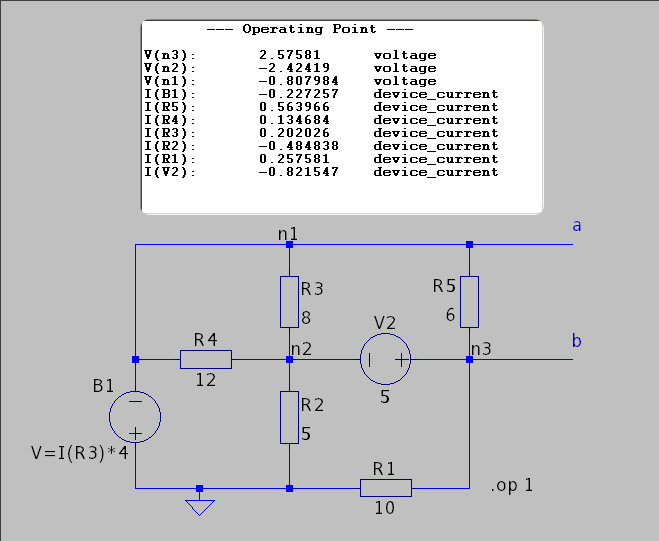
\includegraphics[scale=0.5]{./Figures/ltspice.png} 
\caption{Ltspice simulation 1} 
\label{fig:ltspice_1}
\end{figure}
\clearpage
\subsection{Analytical determination of the Thévenin equivalent}
Now that we have calculated $U_{oc} = U_{th}$ we need to determine the equivalent resistance
$R_{th}$.
Therefore we replace the independent source with its ideal inner resistance and apply a test
volatge $U_T$ at the terminals $a$ and $b$.\\
\begin{figure}[h!] \centering    
\begin{circuitikz}[scale=0.75]
      %controlled Us_1
      \draw (0,0) 
      to[short](0,1)
      to[cvsource, v_=$U_{S_1}$, color=blue]  (0,4)
      to[short, i=$I_{S_1}^?$, color=red](0,5);
      %Us_2
      \draw (10,5) 
      to[short, i=$I_{s_2}^?$, color=red](9,5)
      to[short](5,5);
      %R_1
      \draw                                     (5,0)
      to[short, *-]                             (6,0)
      to[R, l=$R_1$, v<=$U_{R_1}$]              (9,0)
      to[short, i<=$I_{R_1}$, color=red]         (10,0);
      %R_2
      \draw                                     (5,0) 
      to[short]                                 (5,1)
      to[R, l=$R_2$, v<=$U_{R_2}$]              (5,4)
      to[short, i<=$I_{R_2}$, color=red]         (5,5);
      %R_3
      \draw                                     (5,5)
      to[short, *-]                             (5,6)
      to[R, l=$R_3$, v=$U_{R_3}$]              (5,9)
      to[short, i=$I_{R_3}$, color=red]          (5,10)
      to[short, -*]                             (5,10);
      %R_4
      \draw                                     (0,5)
      to[short, *-]                             (1,5)
      to[R, l=$R_4$, v=$U_{R_4}$]               (4,5)
      to[short, i=$I_{R_4}$, color=red]          (5,5);
      %R_5
      \draw                                     (10,5)
      to[short, *-]                             (10,6)
      to[R, l=$R_5$, v=$U_{R_5}$]               (10,9)
      to[short, i=$I_{R_5}$, color=red]          (10,10)
      to[short, -*]                             (10,10);
      %U_T
      \draw                                     (15,5)
      to[short, *-]                             (15,6) 
      to[V, v<=$U_T$, color=blue]               (15,9)
      to[short, i<=$I_T$, color=red]          (15,10)
      to[short, -*]                             (15,10);
      %connections
      \draw (0,5) to[short] (0,10) to[short]    (12.5,10);
      \draw (10,0) to[short] (10,5) to[short]   (12.5,5);
      %clamps + connections
      \draw (12.5,10) to[short, o-] (15,10);
      \draw (12.5,5) to[short, o-] (15,5);
      %ref node
      \draw (5,0) to[short]                             (0,0);
      %grnd
      \draw (0,0) to (0,0) node[ground]{};
      %nodes
      \node[above, color=blue]              (n_1) at (5,10) {$n_1$};
      \node[above, xshift=3mm, color=blue]  (n_3) at (5,5) {$n_2$};
      \node[above, xshift=3mm, color=blue]  (n_4) at (10,5) {$n_3$};
      \node[below, color=blue]              (ref) at (5,0) {ref};
      \node[above]              (a) at (12.5,10) {a};
      \node[above]              (b) at (12.5,5) {b};
      \draw[color=blue](5,10) ellipse (150pt and 15pt);
      \draw[color=blue](5,5) ellipse (25pt and 25pt);
      \draw[color=blue](10,5) ellipse (25pt and 25pt);
      \draw[color=blue](2.5,0) ellipse (80pt and 15pt);
      \draw[color=blue](0,7.5) ellipse (12pt and 80pt);
      \draw[-{Latex[length=2mm]}, color=blue] (-1, 7.5) -- (-1, 0.5)
      node[pos=0.25, left] {$U_{n_1}$};
      \draw[-{Latex[length=2mm]}, color=blue] (4.25, 4.25) -- (2.5, 0.6)
      node[pos=0.45, left] {$U_{n_2}$};
      \draw[-{Latex[length=2mm]}, color=blue] (9.25, 4.25) -- (5.25, 0.25)
      node[pos=0.5, right] {$U_{n_3}$};
\end{circuitikz}
\caption{Network with testvoltage}
\label{fig:Testvoltage}
\end{figure}
\\ We simply add $U_T$ to our Matrix and set $U_{S_2}$ to zero, as it is deactivated.
\begin{equation}
      \begin{pmatrix}
            G_3 + G_4 + G_5 & -G_3 - G_4 & -G_5 & 0 & -1 &1\\
            -G_3 -G_4 & G_2 + G_3 + G_4 & 0 & -1 & 0 &0\\
            -G_5 & 0 & G_1 + G_5 & 1 & 0 &-1\\
            0 & -1 & 1 & 0 & 0 &0\\
            -\alpha G_3-1 & \alpha G_3 & 0 & 0 & 0 &0\\
            1 & 0 & -1 & 0 & 0 & 0\\
      \end{pmatrix}
      \cdot
      \begin{pmatrix}
            U_{n_1}\\U_{n_2}\\U_{n_3}\\I_{s_2}^?\\I_{s_1}^?\\I_T
      \end{pmatrix}
      =
      \begin{pmatrix}
            0\\0\\0\\0\\0\\U_T
      \end{pmatrix}
\end{equation}
After we have calculated the current $I_{T}$, we can calculate the equivalent resistance $R_{th}$
using ohm's law. 
\subsection{Matlab}
\subsubsection{Source code}
\lstinputlisting[language=matlab]{./../matlab/calculations_ass2_2.m}  
\subsubsection{Console output}
\lstinputlisting[language=matlab]{./../matlab/console_output_2.txt}  

\subsection{Numerical results of the Thévenin equivalent}
The open-circuit current $U_{oc}$ resembles our thévenin voltage $U_{th} = -3.3838 V$.
In order to calculate the equivalent resistance, we apply a test voltage $U_{T} = 1V$, which yielded
\[
I_{T} = -0.825A
.\] 
and under consideration of the passive sign convention, we get
\[
R_{th} = \frac{U_{Rnet}}{I_{R}} = \frac{-U_{T}}{I_{T}}= 1.2121\Omega
.\]
\clearpage
\subsection{Ltspice simulation}
To show that our calculations are correct, we first confirm the test-voltage-method. 
\begin{figure}[h!]\centering
   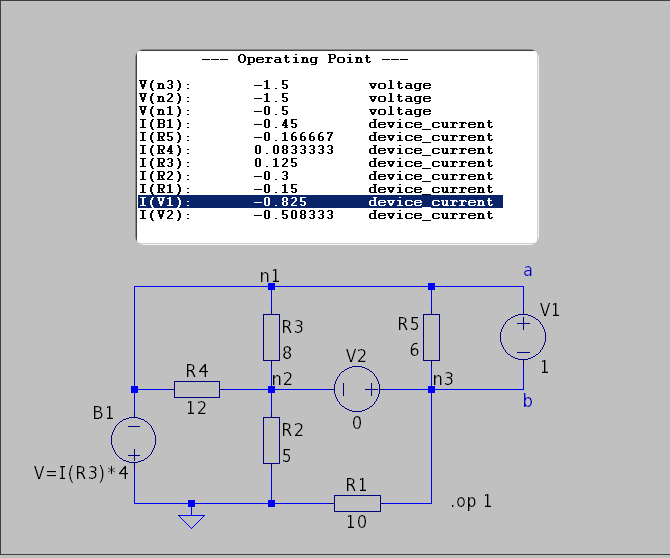
\includegraphics[scale=0.5]{./Figures/ltspice_testvoltage.png} 
\caption{Ltspice simulation 2}
\label{fig:ltspice_2}
\end{figure}
\\Here is the behaviour of the whole circuit as shown in Figure \ref{fig:circuit_assignment2},
\begin{figure}[h!]\centering
   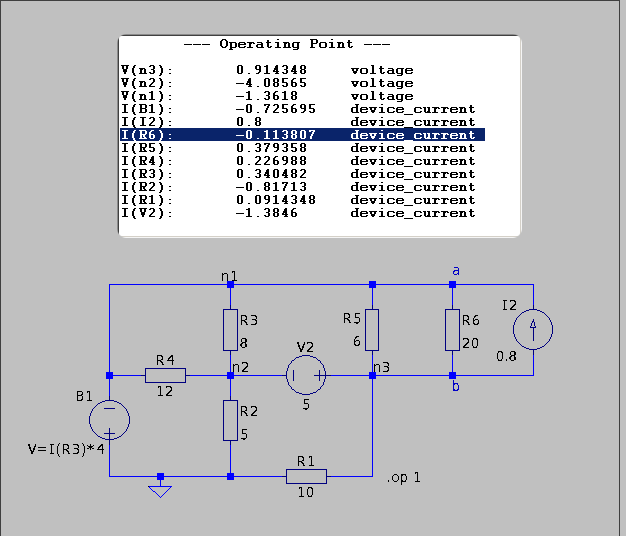
\includegraphics[scale=0.5]{./Figures/ltspice_all.png} 
\caption{Ltspice simulation 3}
\label{fig:ltspice_3}
\end{figure}
\clearpage
And here is the behaviour of its thévenin equivalent. They have the same voltages and currents after
the clamps.
($U_{n1} -U_{n3}$ to get the voltage between $a$ and $b$) 
\begin{figure}[h!]\centering
   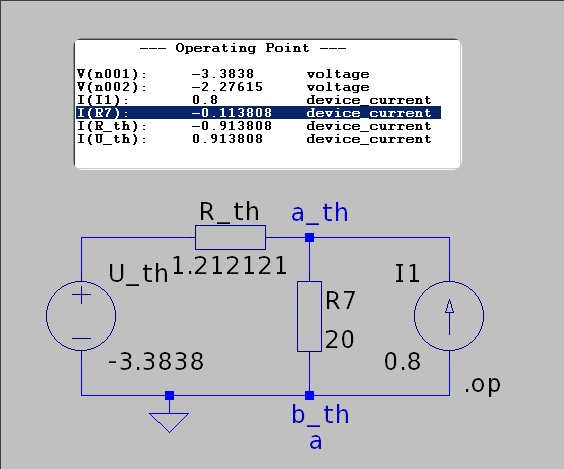
\includegraphics[scale=0.5]{./Figures/ltspice_equivalent.png} 
\caption{Ltspice simulation 4}
\label{fig:ltspice_4}
\end{figure}
\newpage
\subsection{Bonus}
\subsubsection{Network}
\begin{figure}[h!] \centering    
      \begin{circuitikz}[scale=0.75]
            %controlled Us_1
            \draw (0,0) 
            to[short](0,1)
            to[V, v=$U_{TH}$, color=blue]  (0,4)
            to[short, i=$I_{TH}$, color=red](0,5);
            %Is_3
            \draw (10,0) to[I, i=$I_{s_3}$, color =red]        (10,5);
            %R_TH
            \draw                                     (0,5)
            to[short]                             (1,5)
            to[R, l=$R_{TH}$, v=$U_{R_{TH}}$]               (4,5)
            to[short]          (5,5);
            %R_6
            \draw                                     (7,0)
            to[short, *-]                             (7,1) 
            to[R, l=$R_6$, v=$U_{R_6}$]               (7,4)
            to[short, i=$I_{R_6}$, color=red]          (7,5)
            to[short, -*]                             (7,5);
            %clamps + connections
            \draw (5,5) to[short, o-] (10,5);
            \draw (5,0) to[short, o-] (10,0 );
            %ref node
            \draw (5,0) to[short]                             (0,0);
            %grnd
            \draw (0,0) to (0,0) node[ground]{};
            %nodes
            \node[above]              (a) at (5,5) {a};
            \node[above]              (b) at (5,0) {b};
      \end{circuitikz}
      \caption{Thevenin Network}
      \label{fig:Thevenin_nw}
      \end{figure}

      \subsection{Analytical results}
      As we have a linear circuit we need to calculate two relations between $I_{s_3}$ and $U_{R_6}$.
      Then we can set up a linear function in order to determine the right value for $I_{s_{3_{new}}}$.\\
      First we coose 0mA for $I_{s_3}$, so its basicly deactivated:
      \begin{equation}
            U_{R_{6_0}} = U_{TH} + U_{R_{TH}}
      \end{equation}\label{eqn:0mA}
      Then we coose 5mA for $I_{s_3}$. Now there are two sources, so we make use of the principle of
      superposition. We already know the result, if $I_{s_3}$ is deactivated from above, so we 
      just have to deactivate $U_{TH}$.
      \begin{equation*}
            I_{R_{6_5}} = I_{s_3} \cdot \frac{R_{TH}}{R_{TH} + R_6}
      \end{equation*}
      \begin{equation}
            U_{R_{6_{5u}}} = I_{R_{6_5}} \cdot R_6
      \end{equation}\label{eqn:5mA}
      Now we can superpose the result of \ref{eqn:0mA} and \ref{eqn:5mA}:
      \begin{equation}
            U_{R_{6_5}} = U_{R_{6_{5u}}} + U_{R_{6_0}}
      \end{equation}
      With these results we can set up the following function:
      \begin{equation}\label{eqn:function}
            U_{R_{6}} = k \cdot I_{s_{3}} + d
      \end{equation}
      With the function \ref{eqn:function} we can calculate $I_{s_{3_{new}}}$.
\end{document}
